\documentclass[onecolumn,draftcls]{IEEEtran}

% Required packages for math and citations
\usepackage{amsmath, amssymb, amsfonts}
\usepackage{physics}
\usepackage{cite}
\usepackage{datetime}
\usepackage{setspace}
\usepackage{totcount}
\usepackage{comment}
\usepackage{tikz}
\usetikzlibrary{calc,patterns,angles,quotes,decorations.pathmorphing}
% Load tikz before standard LaTeX packages like graphicx
\usepackage{graphicx}


\bibliographystyle{ieeetr}
\doublespacing


% --- Document Information ---
\title{Honors Thesis\\
\large{Literature Review: Lagrangian Mechanics and Wind Turbine Blade Bending}}
\author{Dinor Nallbani}


% --- Document Begins ---
\begin{document}
\begin{titlepage}
    \maketitle
    \begin{center}
        \vfill
        \begin{tabular}{ l l }
            \textbf{Chair:} & Emmanuel Branlard \\
            \textbf{Date:}  & \today
        \end{tabular}
        \vfill
    \end{center}
\end{titlepage}
\tableofcontents
\newpage

\section{Abstract}
\subsection*{Objective}
Wind energy is a critical component of the global transition to sustainable energy systems. Offshore wind turbines, in particular, offer an incredible opportunity to move that sustainable energy to a location where higher energy outputs are possible  as "Wind velocity is higher and more dependable at offshore locations" and "offshore wind energy [being] characterized by higher power density" \cite{Desalegn2023onshore}. In order to harness this energy effectively, offshore wind turbines must grow in size and complexity compared to their onshore counterparts. As wind turbine blades increase in size, understanding their dynamic behavior becomes increasingly important for ensuring structural integrity and operational efficiency. To adress this, this literature review aims to establish a theoretical foundation for using Lagragian mechanics to derive equations of motion (EOMs) investigate the aeroelastic stability of wind turbines and how they vary with rotational and wind speeds. The plan is to focus on the second tower mode, which is known to exhibit complex interactions with aerodynamic forces and could impact the overall stability of the turbine structure. Deriving symbolic EOMs that can capture the complex interactions between aerodynamic forces and structural responses will provide valuable insights into the design and operation of large-scale wind turbines.

\subsection*{Methods}
The primary method this work uses to describe the motion of the systems will be the Lagrange method for analyzing system mechanics. The method uses the principle of least action and an energy-based approach to derive a method for analyzing complex systems in an easier way than using the basic $F=ma$ approach used in Newtonian mechanics \cite{Branlard2025notes}. In Lagrangian mechanics, the Euler-Lagrange equation as well as a function known as a Lagrangian is used to calculate the equations of motion of a system. The equation and Lagrangian are as follows:

\begin{equation}
    \label{eq:lagrange}
    \frac{d}{dt}\left(\frac{\partial\mathcal{L}}{\partial\dot{q}_i}\right)-\frac{\partial\mathcal{L}}{\partial q_i}=Q_{i,nc}
\end{equation}

\begin{equation}
    \label{eq:lagrangian}
    \mathcal{L}=\mathcal{T}-\mathcal{V}
\end{equation}

Where $\mathcal{T}$ is the total kinetic energy of the system, $\mathcal{V}$ is the total potential energy of the system, $q_i$ refers to the set of generalized coordinates, and $Q_{i,nc}$ are the generalized forces acting in those coordinate directions (the degrees of freedom) \cite{Branlard2025notes}. The generalized forces also include the damping forces that act upon the system such as friction, air resistance, and heat generation. Taking the damping forces out of the generalized forces and simplifying the Euler-Lagrange equation leaves us with the following:

\begin{equation}
    \label{eq:euler_lagrange}
    \frac{d}{dt}\left(\frac{\partial\mathcal{T}}{\partial\dot{q}_i}\right)-\frac{\partial\mathcal{T}}{\partial q_i}+
    \frac{\partial\mathcal{T}}{\partial q_i}+
    \frac{\partial\mathcal{D}}{\partial\dot{q}_i} =
    Q_{i}
\end{equation}

Where D is the damping energy in the system.

Lagrangian Mechanics was chosen for this situation as it allows for easier analysis of the complex systems being tackled as well as its usefulness when tackling the bending encountered. The method shines when used on rotating reference frames, similar to the bending of a wind turbine blade when acted upon by the force of wind.


\subsection*{Sources}
For this literature review, ten sources were selected to provide a comprehensive theoretical and methodological basis for the following research. These sources comprise foundational lecture notes on structural dynamics and Lagrangian mechanics, ensuring accurate derivation of the equations of motion. A significant portion of the literature focuses on aeroelastic stability tools and frameworks (HAWCStab and YAMS) which serve as benchmarks for the proposed symbolic analysis. Specific studies addressing damping estimation, modal dynamics, and instability phenomena, such as flutter and stall-induced vibrations, were included to contextualize the physical behaviors of the second tower mode. Finally, recent literature on offshore wind trends was selected to explain the broader motivation for investigating larger, more flexible turbine structures. Collectively, these sources were chosen for their direct relevance to the thesis goal of deriving and linearizing symbolic equations of motion for wind turbine dynamics.

\subsection*{Findings}
First-order modes of wind turbines are well-documented and standard in design load cases, higher-order modes remain a critical area of study that can significantly impact turbine stability. Specifically, the second tower mode involves some sophisticated modeling to accurately capture the dynamic behavior of the tower as it interacts with aerodynamic forces. The literature identifies that these higher-order modes can exhibit low or even negative damping under certain operational conditions, leading to potential aeroelastic instabilities such as flutter or stall-induced vibrations \cite{hansen2007aeroelastic}. Understanding and predicting these behaviors is essential for the safe and efficient operation of large offshore wind turbines, which are increasingly flexible due to their size.

To address the complexities of these higher-order dynamics, the literature emphasizes the utility of symbolic computational frameworks over purely numerical solvers. Recent work demonstrates that symbolic frameworks, such as those implemented in Python using Kane's method or Lagrange's equations, allow for the generation of "glass-box" models where the underlying physical relationships remain transparent \cite{branlard2022symbolic}. These frameworks enable the derivation of equations of motion that can be analytically linearized, facilitating a more direct stability analysis compared to high-fidelity simulations \cite{branlard2022symbolic}. Furthermore, symbolic approaches allow for the creation of models with variable levels of fidelity, which is crucial for isolating the specific effects of the second tower mode without the computational cost of full finite element methods.


\newpage

\section{Introduction}
\subsection*{Motivation}
The global transition toward sustainable energy systems has placed wind energy at the forefront of power generation technologies. To meet growing energy demands and maximize efficiency, the industry is increasingly shifting focus from land-based systems to offshore environments. This transition is driven by the physical advantages of the maritime environment; specifically, offshore wind has a higher potential for energy production than its onshore counterpart. \cite{Desalegn2023onshore}. While offshore systems currently face challenges regarding a higher levelized cost of energy (LCOE) and distinct life-cycle impacts, the potential for optimal power generation continues to drive rapid technological development in this sector \cite{Desalegn2023onshore}. Offshore wind offers a few key advantages over onshore wind resulting from some fundamental physical principles:

The available power in the wind, $P$, increases dramatically with the wind speed, $v$:
\begin{equation}
    \label{eq:power_wind}
    P \propto v^{3}
\end{equation}

Furthermore, the power capture is directly proportional to the area swept by the blades, which scales with the square of the blade length, $r$:
\begin{equation}
    \label{eq:power_area}
    A \propto r^{2}
\end{equation}
Thus, small increases in wind speed or blade length yield significant gains in power output, necessitating larger rotor diameters.

This means the more consistant, higher speed wind occuring farther in the ocean can produce significantly more power than the typically lower and more turbulent onshore winds due to equation \ref{eq:power_wind}. Offshore locations benefit from reduced surface roughness and fewer obstructions, leading to more stable wind profiles. To more effectively harness these lower-turbulence, high-velocity wind resources, wind turbine designs have scaled up dramatically. Modern offshore turbines feature significantly longer blades and taller towers to take advantage of faster with and the power increase that results from equation \ref{eq:power_area}.
However, this geometric upscaling introduces a critical engineering challenge: structural flexibility. Unlike the stiffer, smaller models of the past, modern multi-megawatt turbines are highly flexible structures. This increased flexibility introduces complex aeroelastic phenomena—interactions between aerodynamic forces and structural motion—that are not present or are negligible in rigid systems. As these structures become lighter and more slender to reduce material costs, ensuring their stability against phenomena such as flutter and stall-induced vibrations becomes a primary design constraint \cite{hansen2007aeroelastic}.


\subsection*{Problem Statement}
Aeroelastic studies often prioritize the analysis of fundamental structural modes, such as the first fore-aft tower bending and the first blade flapwise modes, as these contribute most significantly to the overall deflection and load envelope. However, as turbines become larger for offshore purposes, they also become less rigid. Higher-order modes, such as the second tower mode, start to gain prominence in influencing the dynamic response of the structure. These higher-order modes can exhibit very low or even negative aerodynamic damping under specific operational conditions, significantly increasing the risk of aeroelastic instabilities such as stall-induced vibrations or classical flutter \cite{hansen2007aeroelastic}. Moreover, unlike the fundamental modes, the damping mechanisms for the second tower mode are often non-intuitive, arising from complex aeroelastic couplings with the rotor that vary non-linearly with rotational speed and pitch settings \cite{hansen2007aeroelastic}.

Despite the complexity of these modes, current industry-standard tools for analyzing them often rely on high-fidelity, numerical simulators. While accurate, these tools often obscure the underlying mathematical relationships governing the system's behavior, making it difficult to isolate the root causes of instability. Symbolic modeling approaches, which derive equations of motion analytically, offer a promising alternative. Symbolic methods allow a clearer understanding of how different parameters influence the dynamic behavior of the system, enabling engineers to recognize patterns and trends that may not be immediately apparent in the numerical results of the simulation programs \cite{branlard2022symbolic}. They may make it easier to trace how parameters such as rotational speed and wind velocity affect the frequency and damping characteristics of higher-order modes like the second tower mode.

In this thesis, the goal is to use symbolic derivation techniques based on Lagrangian mechanics to systematically develop models of reduced-order wind turbine models of increasing complexity. The primary objective is to isolate and analyze the aeroelastic behavior of the second tower mode, which becomes critical as turbine flexibility increases. By generating these analytical models, this study aims to find the fundamental trends governing how system frequencies and damping ratios evolve as functions of rotor rotational speed and wind velocity.


\newpage

\section{Foundations of Wind Turbine Modeling}
\subsection*{Foundations of Structural Dynamics in Wind Energy}
The modeling of rotating flexible systems, such as wind turbines, requires a robust mechanical framework capable of handling complex kinematic chains.
At first, Newtonian mechanics provides a straight forward approach to analyzing the motion of particles and rigid bodies through equations of motion derived from Newton's second law.

\begin{equation}
    \label{eq:newton}
    F = m\derivative{v}{t}
\end{equation}

However, Newtonian mechanics can become overly complex when applied to multibody systems with varying constraints and rotating reference frames. Instead, the Lagrangian approach as described in equation \ref{eq:lagrange} is far preferred for these applications. The method's reliance on kinetic energy ($\mathcal{T}$) and potential energy ($\mathcal{V}$) bypasses the need to  calculate constraint forces at every joint, streamlining the derivation of the Equations of Motion (EOM) \cite{Branlard2025notes}. This energy-based formulation is advantageous for wind turbine aeroelasticity, where multiple bodies (tower, nacelle, hub, blades) interact dynamically, allowing for a systematic assembly of the system's total energy to derive the governing differential equations.

A central component of this dynamic analysis is accurately defining the system kinematics, specifically through the use of coordinate transformations. To model the motion of a wind turbine blade relative to the ground, it is essential to establish a hierarchy of coordinate systems, starting with an inertial frame fixed to the ground. Any following frames are defined relative to the frames preceeding them as the components all rotate and translate. Following the chain of transformations from the inertial frame throught the chain of bodies all the way to the blade tip allows for precise tracking of positions and velocities of all points on the structure \cite{Branlard2025notes}. This hierarchical approach to coordinate systems is crucial for capturing the complex interactions between aerodynamic forces and structural responses, particularly when analyzing higher-order modes like the second tower mode.

\subsection*{Modeling Approaches}
An important part when modeling wind turbine dynamics is reducing the system into a mathematically manageable form. To achieve this, the Rayleigh-Ritz method, a numerical method of approxamating eigenvalues, is often used to simplify the extremely high number of degrees of freedom present in a flexible structure. By assuming that the deflection of a flexible component, such as a tower or blade, can be represented as a linear combination of known spatial shape functions multiplied by time-dependent generalized coordinates, the system is discretized into a finite set of modes. This transformation converts the governing Partial Differential Equations (PDEs) of the continuous system into a finite set of Ordinary Differential Equations (ODEs) changing "the infinite number of DOF necessary to describe a flexible body onto a reduced and converging set of
shape functions" \cite{branlard2019flexible}

These reduced-order models offer a balance between computational efficiency with physical accuracy, allowing for the simulation of complex turbine behaviors without the high computational demands — and resulting high hardware costs and compute times — of full finite-element analysis. By utilizing shape functions that approximate the mode shapes of the structure, these reduced-order models can capture the essntial dynamics of the system and accurately predict the low-frequency dynamics that dominate the fatigue and stability loads of operational turbines \cite{branlard2019flexible}.

Although the theory is well-known, deriving these equations by hand is tedious and prone to mistakes. To solve this, the use of symbolic computing tools could offer an advantage. Unlike numerical solvers that use approximate numbers, symbolic computing manipulated mathmatical expressions in their exact form. This provides mathematically more precise equations for complex, rotating turbine parts without the risk of human error.

Furthermore, employing symbolic frameworks enables the development of analytical models that serve as a rigorous benchmark for verifying the stability predictions of high-fidelity simulators. For instance, \cite{riva2013analytical} utilized symbolic computation to construct a flexible wind turbine model. By systematically deriving these equations of motion, it becomes possible to isolated specific structural behaviors, such as the variations in tower modes, allowing for a clearer understanding of the root causes of instability compared to numerical simulations \cite{riva2013analytical}.

\subsection*{Aeroelastic Stability and Damping}
As wind turbine structures become increasingly flexible, they become susceptible to a range of aeroelastic instabilities that can compromise structural integrity. Hansen categorizes these instability mechanisms into distinct phenomena, with stall-induced vibrations and classical flutter being among the critical risks for modern turbines \cite{hansen2007aeroelastic}. While blade modes typically benefit from high aerodynamic damping due to their large surface area interacting directly with the airflow, tower modes present a challenge. In conditions where the turbine enters stall, the damping can become negative, leading to self-excited vibrations that grow in amplitude until failure or control intervention occurs \cite{hansen2007aeroelastic}.

Quantifying this damping during actual turbine operation is important information when analyzing stability. Unlike frequency, which can be identified relatively easily from spectral data, damping is harder to estimate accurately from operational data due to wind excitation and the coupling between different structural modes. Hansen et al. highlight these difficulties in their study on operational modal analysis, noting that distinguishing the specific damping values for tower modes often requires sophisticated stochastic techniques \cite{hansen2006two}. Because experimental validation is complex, there is a strong reliance on theoretical models to predict these damping values. This underscores the benefits of the symboling modeling approach proposed in this thesis, which aims to provide a deep understanding of the fundemental trends in turbine dynamics.

A critical aspect of analyzing the second tower mode is understanding its interaction with the rotating rotor, a phenomenon known as "whirling." When the tower bends, it does not oscillate in isolation; the rotation of the rotor creates a gyroscopic coupling that splits the tower's natural frequencies. Hansen et al. explain that this interaction results a backward whirl and a forward whirl \cite{hansen2003improved}. This frequency split is highly sensitive to the rotational speed of the turbine. Capturing these dependencies accurately is essential for predicting the dynamic response of the tower under various operating conditions. The symbolic derivation of the equations of motion, as proposed in this thesis, will facilitate a clear understanding of how these frequency and damping characteristics evolve with rotor speed and wind conditions.

\section{Project Evaluation and Management}

\subsection*{Evaluation}
The success of this Honors Thesis will be evaluated based on the completion of both a Research Manuscript and functional computational models. Specifically, the research committee, chaired by Professor Branlard, will assess the work based on measurable goals. These include the successful symbolic derivation of Equations of Motion for wind turbine models of increasing complexity, and the analytical validation of the frequency and damping trends within these models. Progress will be assessed iweekly through the review of derived equations and code snippets. The final Research Manuscript will be judged on its ability to clearly explain the mathematical trends observed in the computational model.

\subsection*{Communication}
To ensure consistent progress, I will maintain a regular meeting schedule with my faculty sponsor, Professor Branlard. Meetings will be held weekly or bi-weekly for approximately 30, focusing on mathematical derivation issues, reviewing code logic in the Python models, and setting short-term goals for the subsequent week. Between these meetings, I plan to dedicate approximately 10 hours per week to research, coding, and writing to maintain the necessary pace for completion.

\subsection*{Timeline}
From January through March, I will continue work on the Honors Thesis, ensuring that research results are reviewed continuously during weekly meetings. The formal writing process will proceed iteratively, aiming to create a draft of the Research Manuscript by March 13th for the Thesis Committee to review. Following this review, I will deliver my final presentation to the Thesis Committee in April. All the while I intend to refine the computational models and finalize the written manuscript.The properly formatted Research Manuscript along with the associated Python repository, will be submitted via CHC Paths by the end of classes.

\section{Methods}
To achieve the objectives of this thesis, I will be using the sympy library in Python to perform the symbolic derivation of the equations of motion. This process will begin with a familiarization of the library with progressively more complex systems. I will start by deriving the equations of motion for a simple pendulum, a model that has been well-studied, to ensure I can correct apply the framework. Establishing a systematic approach to the derivation process will help ensure the following equations are accurate.

\subsection*{Simple Pendulum}
The inital step will be deriving the equiations of motion of a simple pendulum using Lagrangian mechanics. This will serve as a concept for the symbolic derivation process and allow for the validation of the method against known results. I will derive the equations for both a point mass suspended at the end of the pendulum and a rigid body pendulum.

\begin{figure}[htbp]
    \centering
    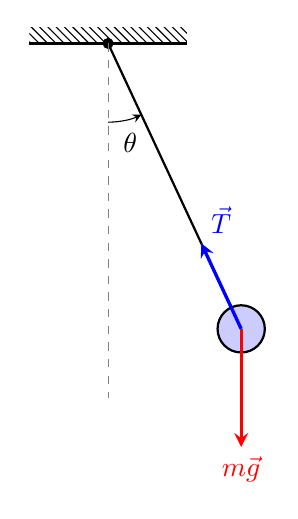
\begin{tikzpicture}[>=stealth]
        % --- 1. Define Core Parameters ---
        \def\L{4}
        \def\angleVal{25}

        % --- 2. Define Coordinates ---
        \coordinate (O) at (0,0);
        \coordinate (V) at (0,-\L-0.5);
        \coordinate (Bob) at ({\L*sin(\angleVal)}, {-\L*cos(\angleVal)});

        % --- 3. Draw the Structure ---
        \draw[line width=1.2pt] (-1,0) -- (1,0);
        \fill[pattern=north west lines] (-1,0) rectangle (1,0.2);
        \fill (O) circle (2pt);

        \draw[thick] (O) -- (Bob);
        \filldraw[fill=blue!20,draw=black,thick] (Bob) circle (0.3);

        % --- 4. Draw Reference Lines ---
        \draw[dashed,gray] (O) -- (V);

        % --- 5. Draw the Angular Coordinate (theta) ---
        \pic [draw=black,->, "$\theta$", angle eccentricity=1.3, angle radius=1cm] {angle = V--O--Bob};

        \def\vecScale{1.5}

        % --- A. Tension Force (T) ---
        \draw[->,blue,very thick] (Bob) -- ($(Bob)!1.2cm!(O)$);
        \node[anchor=south west,blue] at ($(Bob)!1.2cm!(O)$) {$\vec{T}$};

        % --- B. Gravitational Force (mg) ---
        \coordinate (G) at ($(Bob)+(0,-\vecScale)$);
        \draw[->,red,very thick] (Bob) -- (G);
        \node[anchor=north,red] at (G) {$m\vec{g}$};

        % % --- C. Decomposition of mg ---
        % \coordinate (Gradial) at ($(O)!(G)!(Bob)$);
        % % \draw[dashed,gray] (G) -- (Gradial);
        % \draw[->,red!50!black,thick] (Bob) -- (Gradial) node[midway,right,xshift=2pt] {\scriptsize $mg\cos\theta$};

        % \coordinate (Gtangential) at ($(Bob)!(G)!($(Bob)+({\angleVal-180}:1)$)$);
        % \draw[->,red!50!black,thick] (Bob) -- ($(Bob)!0.8!(Gtangential)$) node[anchor=center, xshift=-11, yshift=-5pt] {\footnotesize $mg\sin\theta$};

        % --- 7. Label Mass ---
        % \node at (Bob) {$m$};
    \end{tikzpicture}
    \caption{Free Body Diagram of a simple pendulum with a point mass. The generalized coordinate $\theta$ is defined relative to the vertical, and the two primary forces are the tension $\vec{T}$ and gravity $m\vec{g}$, which contains a radial ($mg\cos\theta$) and tangential ($mg\sin\theta$) component.}
    \label{fig:pendulum_fbd}
\end{figure}

\subsubsection*{Point Mass}
The point mass pendulum is the simplest form of a pendulum, where all the mass is concentrated at a single point at the end of a massless rod. Applying the Euler-Lagrange equation will result in the well-known nonlinear equation of motion for the simple pendulum

\begin{equation}
    \label{eq:pendulum_point_mass}
    \ddot{\theta} + \frac{g}{l} \sin\theta = 0
\end{equation}

\subsubsection*{Rigid Body}
Using a slightly more complex model, the rigid body pendulum, allows for the calculation of the moment of inertia and distribution of mass along the length of the pendulum. This will yield a more complex equation of motion that accounts for the rotational inertia of the pendulum, providing a more accurate representation of its dynamics. In my model, I assumed the rod is a rectangle with uniform mass distribution, which allows for the calculation of the moment of inertia as $I = \frac{1}{3}ml^2$ from the end of the rod. The resulting equation of motion is:

\begin{equation}
    \label{eq:pendulum_rigid_body}
    \ddot{\theta} + \frac{3g}{2l} \sin\theta = 0
\end{equation}

\subsection*{Double Pendulum}
The same processes were applied to a double pendulum, two pendulums attached end to end. This systems is another well known system, making it another good proof of concept for the symbolic derivation process. The equations of motion for the double pendulum are more complex than the simple pendulum, as they involve the interaction between the two masses and their respective angles. The angles are $\theta_1$ and $\theta_2$ calculated relative to the previous angle.

\begin{figure}[htbp]
    \centering
    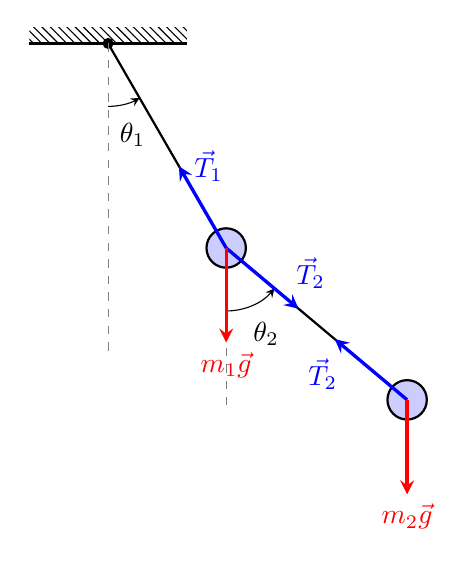
\begin{tikzpicture}[>=stealth]
        % --- 1. Define Core Parameters ---
        \def\L{3}
        \def\thetaOne{30}
        \def\thetaTwo{50}
        \def\vecScale{1.2}

        % --- 2. Define Coordinates ---
        \coordinate (O) at (0,0);
        \coordinate (Bob1) at ({\L*sin(\thetaOne)}, {-\L*cos(\thetaOne)});
        \coordinate (Bob2) at ($(Bob1) + ({\L*sin(\thetaTwo)}, {-\L*cos(\thetaTwo)})$);

        % Reference verticals
        \coordinate (V1) at (0,-1.5);
        \coordinate (V2) at ($(Bob1) + (0,-1.5)$);

        % --- 3. Draw the Structure ---
        \draw[line width=1.2pt] (-1,0) -- (1,0);
        \fill[pattern=north west lines] (-1,0) rectangle (1,0.2);
        \fill (O) circle (2pt);

        \draw[thick] (O) -- (Bob1);
        \draw[thick] (Bob1) -- (Bob2);

        \filldraw[fill=blue!20,draw=black,thick] (Bob1) circle (0.25) node {};
        \filldraw[fill=blue!20,draw=black,thick] (Bob2) circle (0.25) node {};

        % --- 4. Reference Lines and Angles ---
        \draw[dashed,gray] (O) -- (0,-4);
        \draw[dashed,gray] (Bob1) -- ($(Bob1) + (0,-2)$);

        \pic [draw=black,->, "$\theta_1$", angle eccentricity=1.5, angle radius=0.8cm] {angle = V1--O--Bob1};
        \pic [draw=black,->, "$\theta_2$", angle eccentricity=1.5, angle radius=0.8cm] {angle = V2--Bob1--Bob2};

        % --- 5. Forces on Mass 1 ---
        % Tension T1 (Upwards)
        \draw[->,blue,very thick] (Bob1) -- ($(Bob1)!1.2cm!(O)$);
        \node[anchor=west,blue,xshift=2pt] at ($(Bob1)!1.2cm!(O)$) {$\vec{T}_1$};

        % Tension T2 reaction (Downwards along rod 2)
        \draw[->,blue,very thick] (Bob1) -- ($(Bob1)!1.2cm!(Bob2)$);
        \node[anchor=south west,blue] at ($(Bob1)!1cm!(Bob2)$) {$\vec{T}_2$};

        % Gravity m1g
        \draw[->,red,very thick] (Bob1) -- +(0,-\vecScale);
        \node[anchor=north,red] at ($(Bob1)+(0,-\vecScale)$) {$m_1\vec{g}$};

        % Tension T2 (Upwards along rod 2)
        \draw[->,blue,very thick] (Bob2) -- ($(Bob2)!1.2cm!(Bob1)$);
        \node[anchor=north east,blue] at ($(Bob2)!1cm!(Bob1)$) {$\vec{T}_2$};

        % Gravity m2g
        \draw[->,red,very thick] (Bob2) -- +(0,-\vecScale);
        \node[anchor=north,red] at ($(Bob2)+(0,-\vecScale)$) {$m_2\vec{g}$};

    \end{tikzpicture}
    \caption{Free Body Diagram of a double pendulum. The coordinates $\theta_1$ and $\theta_2$ are defined relative to the vertical. Mass $m_1$ is acted upon by gravity $m_1\vec{g}$ and the tensions from both rods, while $m_2$ is acted upon by $m_2\vec{g}$ and the tension $\vec{T}_2$.}
    \label{fig:double_pendulum_fbd}
\end{figure}

The resulting equations of motion are shown with the following Matrix Decomposition

\begin{equation}
    \label{eq:matrix_decomposition}
    M \ddot{q} = F
\end{equation}

Where M is the mass matrix, ${q}$ is the vector of generalized coordinates, and F is the vector of generalized forces. The equations of motion for the double pendulum can be expressed in this form, allowing for a more systematic analysis of the system's dynamics.

\subsubsection*{Point Mass} The Matrix Decomposition for the double pendulum with point masses was calculated as follows:

\begin{equation}
    \label{eq:double_pendulum_mass_matrix} M =
    \left[\begin{matrix}l_{1}^{2} \left(m_{1} + m_{2}\right)              & l_{1}
              l_{2} m_{2} \cos{\left(\theta_{1} - \theta_{2} \right)}       \\l_{1} l_{2}
              m_{2} \cos{\left(\theta_{1} - \theta_{2} \right)} & l_{2}^{2}
              m_{2}\end{matrix}\right]
\end{equation}

\begin{equation} \label{eq:double_pendulum_forcing_terms} F =
    \left[\begin{matrix}- l_{1} \left(g m_{1} \sin{\left(\theta_{1} \right)} + g m_{2} \sin{\left(\theta_{1} \right)} + l_{2} m_{2} \sin{\left(\theta_{1} - \theta_{2} \right)} \dot{\theta}_{2}^{2}\right)\\l_{2} m_{2} \left(- g \sin{\left(\theta_{2} \right)} + l_{1} \sin{\left(\theta_{1} - \theta_{2} \right)} \dot{\theta}_{1}^{2}\right)\end{matrix}\right]
\end{equation}


\subsubsection*{Rigid Body}
The Rigid Body double pendulum was also calculated and resulted in different equations of motions. This is due to the differing mass distribution and moment of inertia of the rigid body compared to the point mass. The equations of motion are as follows:

\begin{equation}
    \label{eq:double_pendulum_rigid_mass_matrix} M =
    \begin{bmatrix}
        \frac{1}{3} l_1^2 m_1 + l_1^2 m_2 + l_1 l_2 m_2 \cos\theta_2 + \frac{1}{3} l_2^2 m_2 &
        l_2 m_2 \left(\frac{1}{2} l_1 \cos\theta_2 + \frac{1}{3} l_2\right)                    \\
        l_2 m_2 \left(\frac{1}{2} l_1 \cos\theta_2 + \frac{1}{3} l_2\right)                  &
        \frac{1}{3} l_2^2 m_2
    \end{bmatrix}
\end{equation}

\begin{equation}
    \label{eq:double_pendulum_rigid_forcing_terms} F =
    \begin{bmatrix}
        -\frac{g l_1 m_1 \sin\theta_1}{2} - g m_2 \left(l_1 \sin\theta_1 + \frac{l_2 \sin(\theta_1 + \theta_2)}{2}\right) + \frac{l_1 l_2 m_2 (2 \dot{\theta}_1 + \dot{\theta}_2) \sin\theta_2 \dot{\theta}_2}{2} \\
        -\frac{l_2 m_2 \left(g \sin(\theta_1 + \theta_2) + l_1 \sin\theta_2 \dot{\theta}_1^2\right)}{2}
    \end{bmatrix}
\end{equation}








%TODO 
% non-wind turbines can go in the appendix
% ADD COORDINATE SSYTEMS

% ADD ALL VARIABLES TO TEXT

% DOUBLE CHECK onebladeTN
% add integral to RFBFN
%Finish FTRSB,
% Write velocity and rotational velocity (only for rigid bodies) vectors at every point that's interesting on the blade, at least one per body (COM, POI's)

% Try some of models in openfast (do TNSB and FTRSB when done)
% put into state space for and 
% Intergrate with respect to timme and find theta, psi with initial cond.
% compare w/ openfast results


% PUt in report equation of finite element shape functions for pure translation and pure rotation and expalin them.
%   ideally find equ and put coeff. of polynomial in elastodyne file.






% todo CHANGE THIS NAME
\subsection*{Single Blade, Pendulum on a Cart}
A single blade model, working on increasing complexity, was derived using a 2-DOF "pendulum on a cart" analogy. This model consists of a translational degree of freedom $x$ representing the tower's fore-aft motion, and a rotational degree of freedom $\psi$ representing the azimuth of the blade. The mass is separated into a nacelle mass ($m_n$), and a rotor mass ($m_s + m_b$).

\begin{figure}[htbp]
    \centering
    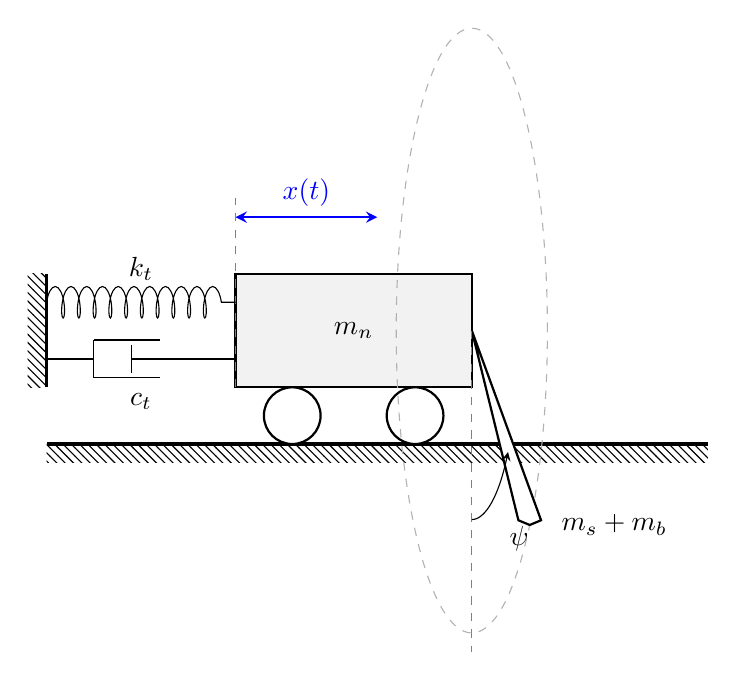
\begin{tikzpicture}[>=stealth, scale=1.2]
        % --- 1. Parameters ---
        \def\cartW{2.5}
        \def\cartH{1.2}
        \def\bladeL{3.2}
        \def\psiAngle{50} 
        
        % --- 2. Draw Ground ---
        \draw[line width=1.2pt] (-2,-0.6) -- (5,-0.6);
        \fill[pattern=north west lines] (-2,-0.6) rectangle (5,-0.8);

        % --- 3. Draw Cart (Nacelle) ---
        \draw[thick, fill=gray!10] (0,0) rectangle (\cartW,\cartH);
        \node at (0.5*\cartW, 0.5*\cartH) {$m_n$};
        
        % Wheels
        \draw[thick, fill=white] (0.6,-0.3) circle (0.3);
        \draw[thick, fill=white] (1.9,-0.3) circle (0.3);
        
        % Displacement x(t)
        \draw[<->, thick, blue] (0, 1.8) -- (1.5, 1.8) node[midway, above] {$x(t)$};
        \draw[dashed, gray] (0,0) -- (0, 2.0);

        % --- 4. Draw Rotor/Blade (Rotating into the page) ---
        \coordinate (Hub) at (\cartW, 0.6); 
        
        % Elliptical path indicating rotation out-of-plane
        \draw[dashed, gray!60] (Hub) ellipse (0.8 and 3.2);
        
        % Define Blade Tip with azimuthal projection
        \coordinate (Tip) at ({\cartW + 0.8*sin(\psiAngle)}, {0.6 - \bladeL*cos(\psiAngle)});
        
        % Tapered Blade Body
        \draw[fill=white, thick] (Hub) -- ($(Tip)+(0.12,0.05)$) -- (Tip) -- ($(Tip)+(-0.12,0.05)$) -- cycle;
        \node[right=8pt] at (Tip) {$m_s + m_b$};

        % Azimuth angle psi 
        \draw[dashed, gray] (Hub) -- ($(Hub)+(0,-3.4)$);
        \draw[->] ($(Hub)+(0,-2.0)$) arc (-90:{-90+\psiAngle}:0.5 and 2.0);
        \node at ({\cartW + 0.5}, -1.6) {$\psi$};

        % --- 5. Stiffness and Damping (Corrected Damper) ---
        \draw[line width=1.2pt] (-2, 0) -- (-2, 1.2);
        \fill[pattern=north west lines] (-2.2, 0) rectangle (-2, 1.2);

        % Spring (kt)
        \draw [decoration={coil, aspect=0.3, segment length=2mm, amplitude=2mm}, decorate] (-2, 0.9) -- (0, 0.9);
        \node at (-1, 1.25) {$k_t$};

        % Damper (ct) - Fixed to use standard drawing commands
        \draw (-2, 0.3) -- (-1.5, 0.3); % from wall
        \draw (-1.5, 0.1) -- (-1.5, 0.5); % cylinder back
        \draw (-1.5, 0.5) -- (-0.8, 0.5); % cylinder top
        \draw (-1.5, 0.1) -- (-0.8, 0.1); % cylinder bottom
        \draw (-1.1, 0.15) -- (-1.1, 0.45); % piston head
        \draw (-1.1, 0.3) -- (0, 0.3); % piston rod to cart
        \node at (-1, -0.15) {$c_t$};
    \end{tikzpicture}
    \caption{Refined 2-DOF model with azimuthal rotation ($\psi$) and tapered blade geometry.}
    \label{fig:one_blade_cart_refined}
\end{figure}

The mass matrix $M$ and forcing vector $F$ were derived symbolically. The rotor center of mass offset ($Y_r, Z_r$) and the rotor inertia ($I_{rxx}$) are included:

\begin{equation}
    \label{eq:cart_mass_matrix} M =
    \begin{bmatrix}
        m_b + m_n + m_s & 0 \\
        0 & I_{rxx} + (Y_{r}^{2} + Z_{r}^{2}) (m_b + m_s)
    \end{bmatrix}
\end{equation}

\begin{equation} 
    \label{eq:cart_forcing_terms} F =
    \begin{bmatrix}
        - c_{t} \dot{x} - k_{t} x \\
        - g (m_b + m_s) (Y_{r} \cos\psi - Z_{r} \sin\psi)
    \end{bmatrix} 
\end{equation}

\subsection*{Tilting Nacelle, Single Blade}
Building upon the previous models, a tilting nacelle model was derived to capture the structural dynamics of a tower with a pitching degree of freedom. This model includes a rotational DOF ($\theta$) representing the fore-aft tilt of the nacelle about a pivot point $O$, and a rotational degree of freedom ($\psi$) representing the azimuth of the blade relative to the nacelle.

\begin{figure}[htbp]
    \centering
    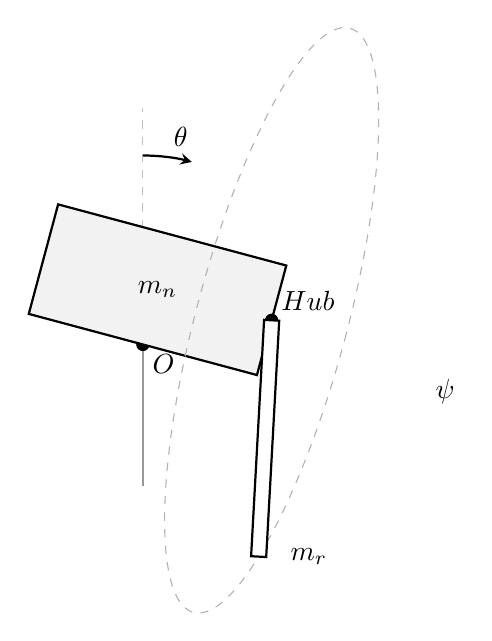
\begin{tikzpicture}[>=stealth, scale=1.2]
        % --- 1. Parameters ---
        \def\tiltAngle{-15} % theta
        \def\towerH{1.5}   
        \def\nacW{2.5}
        \def\nacH{1.2}
        \def\bladeL{3.5}
        \def\psiAngle{40}
        
        % --- 2. Tower Base and Pivot ---
        \draw[thick, gray!80] (0, -\towerH) -- (0, 0);
        \draw[dashed, gray!50] (0, 0) -- (0, 2.5); % Extended vertical reference
        
        \coordinate (O) at (0,0);
        \fill (O) circle (2pt) node[below right] {$O$};

        % --- 3. Tilted Scope ---
        \begin{scope}[rotate around={\tiltAngle:(O)}]
            % Nacelle
            \draw[thick, fill=gray!10] (-\nacW/2, 0) rectangle (\nacW/2, \nacH);
            \node at (0, 0.5*\nacH) {$m_n$};
            
            % Hub point - Moved to the edge (nacW/2 = 1.25)
            \coordinate (Hub) at (1.25, 0.6); 
            \fill (Hub) circle (2pt) node[above right] {$Hub$};

            % Blade path
            \draw[dashed, gray!60] (Hub) ellipse (0.8 and 3.2);
            
            % Tip position
            \coordinate (Tip) at ($(Hub) + ({0.8*sin(\psiAngle)}, {-3.2*cos(\psiAngle)})$);
            
            % Rectangular Blade
            \draw[fill=white, thick] 
                ($(Hub)!0.08cm!90:(Tip)$) -- ($(Tip)!0.08cm!-90:(Hub)$) -- 
                ($(Tip)!0.08cm!90:(Hub)$) -- ($(Hub)!0.08cm!-90:(Tip)$) -- cycle;
            \node[right=8pt] at (Tip) {$m_r$};
        \end{scope}

        % --- 4. Annotations ---
        \draw[->, thick] (0, 2.0) arc (90:{90+\tiltAngle}:2.0);
        \node at (0.4, 2.2) {$\theta$};

        % Azimuth psi reference
        \node at (3.2, -0.5) {$\psi$};
    \end{tikzpicture}
    \caption{Schematic of the Tilting Nacelle model. The hub is positioned at the edge of the nacelle, with the angle $\theta$ representing the tilt and $\psi$ the azimuth.}
    \label{fig:tilting_nacelle_tower_top}
\end{figure}

The mass matrix $M$ and forcing vector $F$ for the tilting nacelle model are expressed below in their full symbolic forms.

\begin{equation}
    \label{eq:tilting_mass_matrix_full}
    \resizebox{0.95\textwidth}{!}{%
    $M = \begin{bmatrix}
        J_{yyN} + J_{yyR} \cos^{2}\psi + J_{zzR} \sin^{2}\psi + m_{n}(X_{n}^{2} + Z_{n}^{2}) + m_{r}(X_{h}^{2} + Z_{h}^{2} + 2 Z_{h} Z_{r} \cos\psi + Z_{r}^{2} \cos^{2}\psi) & X_{h} Z_{r} m_{r} \sin\psi \\
        X_{h} Z_{r} m_{r} \sin\psi & J_{xxR} + Z_{r}^{2} m_{r}
    \end{bmatrix}$%
    }
\end{equation}

\begin{equation} 
    \label{eq:tilting_forcing_terms_full}
    \resizebox{0.95\textwidth}{!}{%
    $F = \begin{bmatrix}
        (J_{yyR} - J_{zzR} + Z_{r}^{2} m_{r}) \sin(2\psi) \dot{\psi} \dot{\theta} - X_{h} Z_{r} m_{r} \cos\psi \dot{\psi}^{2} + (X_{h} m_{r} + X_{n} m_{n}) g \cos\theta + 2 Z_{h} Z_{r} m_{r} \sin\psi \dot{\psi} \dot{\theta} + (Z_{h} m_{r} + Z_{n} m_{n}) g \sin\theta - \frac{Z_{r} g m_{r} \sin(\psi - \theta)}{2} + \frac{Z_{r} g m_{r} \sin(\psi + \theta)}{2} \\
        \left(- J_{yyR} \cos\psi \dot{\theta}^{2} + J_{zzR} \cos\psi \dot{\theta}^{2} - Z_{h} Z_{r} m_{r} \dot{\theta}^{2} - Z_{r}^{2} m_{r} \cos\psi \dot{\theta}^{2} + Z_{r} g m_{r} \cos\theta \right) \sin\psi
    \end{bmatrix}$%
    }
\end{equation}

\subsection*{Rotating Flexible Blade on Fixed Nacelle}
A flexible blade rotating about a fixed nacelle model was developed as a simplified model for flexible blade analysis. This model employs a flexing degree of freedom ($q$) to represent the deflection of the blade, and a rotational degree of freedom ($\psi$) representing the azimuth. The nacelle is assumed to be rigid and stationary for this derivation to isolate the rotation and blade bending.

\begin{figure}[htbp]
    \centering
    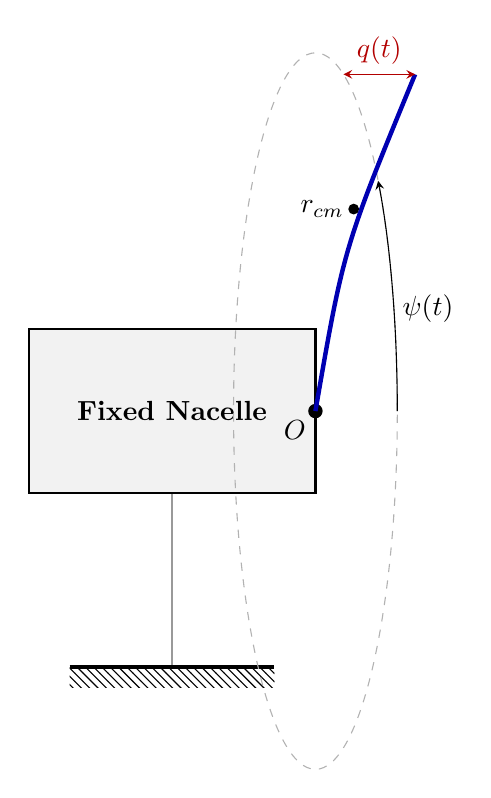
\begin{tikzpicture}[>=stealth, scale=1.3]
        % --- 1. Parameters ---
        \def\nacW{2.8}
        \def\nacH{1.6}
        \def\bladeL{3.5}
        \def\psiAngle{70}    % Azimuth angle
        \def\flexOffset{0.7} % Modal deflection q(t) - flexing left/right
        
        % --- 2. Ground Reference ---
        \draw[thick, gray!80] (0, -0.8) -- (0, -2.5);
        \draw[line width=1.2pt] (-1,-2.5) -- (1,-2.5);
        \fill[pattern=north west lines] (-1,-2.7) rectangle (1,-2.5);

        % --- 3. Fixed Nacelle ---
        % Drawn as a rectangle viewed from the side
        \draw[thick, fill=gray!10] (-\nacW/2, -0.8) rectangle (\nacW/2, 0.8);
        \node at (0, 0) {\textbf{Fixed Nacelle}};
        
        % Hub point (Origin O) at the right edge
        \coordinate (O) at (\nacW/2, 0);
        \fill (O) circle (2pt) node[below left] {$O$};

        % --- 4. Rotating and Flexing Blade (Side-on perspective) ---
        % Elliptical path indicating rotation "into the page"
        \draw[dashed, gray!60] (O) ellipse (0.8 and 3.5);

        % Tip Position: 
        % The vertical (z) component follows sin(psi)
        % The horizontal (x) component is the flexural displacement q(t)
        \coordinate (RefAxis) at ({\nacW/2 + 0.8*cos(\psiAngle)}, {3.5*sin(\psiAngle)});
        \coordinate (Tip) at ({\nacW/2 + 0.8*cos(\psiAngle) + \flexOffset}, {3.5*sin(\psiAngle)});

        % Draw Flexible Blade Body
        % Curves from the hub O to the deflected tip
        \draw[ultra thick, blue!70!black] (O) 
            .. controls ({\nacW/2 + 0.4*cos(\psiAngle) + \flexOffset*0.2}, {1.7*sin(\psiAngle)}) .. (Tip);
        
        % Center of Mass Label (r_cm)
        \fill ({\nacW/2 + 0.8*cos(\psiAngle)*0.6 + \flexOffset*0.3}, {3.5*sin(\psiAngle)*0.6}) circle (1.5pt);
        \node[left] at ({\nacW/2 + 0.8*cos(\psiAngle)*0.6 + \flexOffset*0.3}, {3.5*sin(\psiAngle)*0.6}) {$r_{cm}$};

        % --- 5. Annotations ---
        % Flexural DOF q(t) - Horizontal displacement arrow
        \draw[<->, red!70!black] (RefAxis) -- (Tip) node[midway, above] {$q(t)$};
        
        % Azimuth psi indicator (along the elliptical path)
        \draw[->] ({\nacW/2 + 0.8}, 0) arc (0:40:0.8 and 3.5);
        \node at ({\nacW/2 + 1.1}, 1.0) {$\psi(t)$};
        
    \end{tikzpicture}
    \caption{Side-on perspective of the rotating flexible blade. The blade rotates into the page along an elliptical path ($\psi$), while the modal deflection $q(t)$ occurs horizontally along the x-axis.}
    \label{fig:flexible_blade_side_view}
\end{figure}

The system's kinetic energy consists of rotational components for the hub and blade ($J_{hub}, J_b$) and flexural energy associated with the modal mass ($GM_b$). Potential energy accounts for the elastic restoration of the blade ($K_b$) and gravitational effects on the blade's center of mass ($r_{cm}$). The mass matrix $M$ and forcing vector $F$ are:

\begin{equation}
    \label{eq:flex_blade_mass_matrix} M =
    \begin{bmatrix}
        GM_{b} & 0 \\
        0 & J_{b} + J_{hub}
    \end{bmatrix}
\end{equation}

\begin{equation} 
    \label{eq:flex_blade_forcing_terms} F =
    \begin{bmatrix}
        -K_{b} q(t) \\
        g m_{b} r_{cm} \sin\psi(t)
    \end{bmatrix} 
\end{equation}
This model serves as the basis for calculating the blade's natural frequencies and analyzing how the gravitational load fluctuates as a function of the azimuth $\psi$.

\subsection*{Flexible Tower, Rigid Single Blade}
To increase complexity the model was expanded to include tower flexibility. The tower's first fore-aft bending mode is modeled using a single generalized coordinate ($q_{T1}$). This transition from a simple rigid tilt to a flexible representation involves the use of modal parameters, including the modal mass ($GM_{T11}$), modal stiffness ($K_{eT11}$), and modal damping ($D_{eT11}$). The rotor remains a rigid body with an inertial frame $R$ rotating at an azimuth $\psi$.

\begin{figure}[htbp]
    \centering
    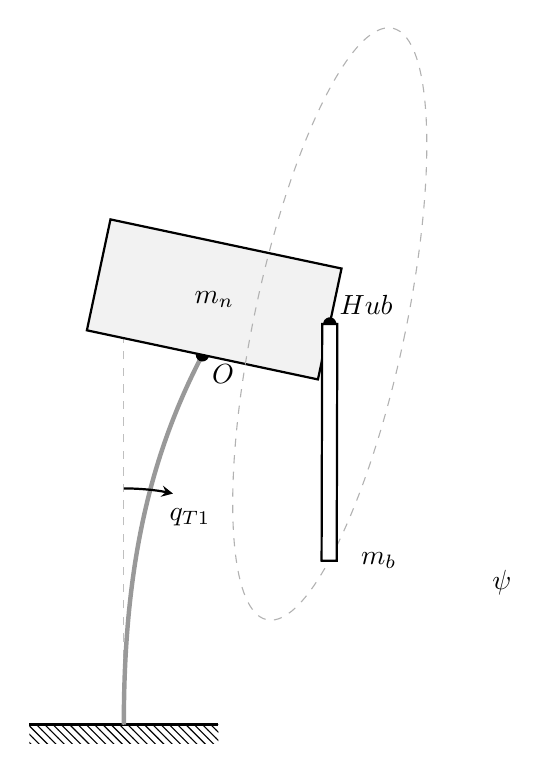
\begin{tikzpicture}[>=stealth, scale=1.2]
        % --- 1. Parameters ---
        \def\deflectionAngle{12} % q_T1
        \def\towerH{4.0}
        \def\nacW{2.5}
        \def\nacH{1.2}
        \def\psiAngle{40}
        
        % --- 2. Ground ---
        \draw[line width=1.2pt] (-1,0) -- (1,0);
        \fill[pattern=north west lines] (-1,0) rectangle (1,-0.2);
        \coordinate (Base) at (0,0);

        % --- 3. Flexible Tower (Bezier Curve) ---
        % Reference vertical
        \draw[dashed, gray!50] (0,0) -- (0, \towerH + 1.0);
        
        % Deflected Tower Shape
        \draw[ultra thick, gray!80] (Base) .. controls (0, \towerH*0.4) and ({0.3*\towerH*sin(\deflectionAngle)}, \towerH*0.7) .. ({ \towerH*sin(\deflectionAngle) }, { \towerH*cos(\deflectionAngle) });
        
        \coordinate (O) at ({ \towerH*sin(\deflectionAngle) }, { \towerH*cos(\deflectionAngle) });
        \fill (O) circle (2pt) node[below right] {$O$};

        % --- 4. Tilted Nacelle Scope (Attached to Tower Top) ---
        \begin{scope}[shift={(O)}, rotate around={-\deflectionAngle:(0,0)}]
            % Nacelle - Centered at O
            \draw[thick, fill=gray!10] (-\nacW/2, 0) rectangle (\nacW/2, \nacH);
            \node at (0, 0.5*\nacH) {$m_n$};
            
            % Hub point
            \coordinate (Hub) at (1.25, 0.6); 
            \fill (Hub) circle (2pt) node[above right] {$Hub$};

            % Blade Path and Rigid Blade
            \draw[dashed, gray!60] (Hub) ellipse (0.8 and 3.2);
            \coordinate (Tip) at ($(Hub) + ({0.8*sin(\psiAngle)}, {-3.2*cos(\psiAngle)})$);
            
            \draw[fill=white, thick] 
                ($(Hub)!0.08cm!90:(Tip)$) -- ($(Tip)!0.08cm!-90:(Hub)$) -- 
                ($(Tip)!0.08cm!90:(Hub)$) -- ($(Hub)!0.08cm!-90:(Tip)$) -- cycle;
            \node[right=8pt] at (Tip) {$m_b$};
        \end{scope}

        % --- 5. Annotations ---
        % Tower Top Rotation q_T1
        \draw[->, thick] (0, 2.5) arc (90:{90-\deflectionAngle}:2.5);
        \node at (0.7, 2.2) {$q_{T1}$};

        % Azimuth psi reference
        \node at (4.0, 1.5) {$\psi$};
    \end{tikzpicture}
    \caption{Schematic of the Flexible Tower model. The tower is represented by a modal deflection $q_{T1}$, which defines both the translation and rotation of the nacelle at point $O$.}
    \label{fig:flexible_tower_model}
\end{figure}

The equations of motion were derived by considering the kinetic energy of the flexible tower, the translating and rotating nacelle, and the rotating rotor. The mass matrix $M$ and forcing vector $F$ are expressed in their full symbolic form below.

\begin{equation}
    \label{eq:flex_tower_mass_matrix}
    \resizebox{0.95\textwidth}{!}{%
    $M = \begin{bmatrix}
        GM_{T11} + J_{yyN} + J_{yyb} \cos^{2}\psi + J_{zzb} \sin^{2}\psi + m_{b}(x_{NB}^{2} + z_{BG}^{2} \cos^{2}\psi + 2 z_{BG} z_{NB} \cos\psi + z_{NB}^{2}) + m_{n}(x_{NG}^{2} + z_{NG}^{2}) & m_{b} x_{NB} z_{BG} \sin\psi \\
        m_{b} x_{NB} z_{BG} \sin\psi & J_{xxb} + m_{b} z_{BG}^{2}
    \end{bmatrix}$%
    }
\end{equation}

\begin{equation} 
    \label{eq:flex_tower_forcing_terms}
    \resizebox{0.95\textwidth}{!}{%
    $F = \begin{bmatrix}
        - D_{eT11} \dot{q}_{T1} + (J_{yyb} - J_{zzb} + m_{b} z_{BG}^{2}) \sin(2\psi) \dot{\psi} \dot{q}_{T1} - K_{eT11} q_{T1} + g m_{b} \dots + m_{b} z_{BG} ( - x_{NB} \cos\psi \dot{\psi} + \dots) \dot{\psi} \\
        \left( - (J_{yyb} - J_{zzb} + m_{b} z_{BG}^{2}) \cos\psi \dot{q}_{T1}^{2} - m_{b} z_{BG} z_{NB} \dot{q}_{T1}^{2} + g m_{b} z_{BG} \cos q_{T1} \right) \sin\psi
    \end{bmatrix}$%
    }
\end{equation}

\section{Conclusion}
The review of current literature shows a clear distinction in the modeling of wind turbine dynamics. On one hand, numerical simulators provide comprehensive data but often obscure the driving physical mechanisms behind complex instabilities. On the other hand, symbolic models have emerged as powerful tools for isolating specific dynamic behaviors \cite{branlard2022symbolic}. These symbolic frameworks are identified as particularly valuable for understanding the fundamental trends of aeroelastic instabilities, such as flutter and stall-induced vibrations, which pose significant risks to the structural integrity of modern, flexible offshore turbines \cite{hansen2007aeroelastic}.

Despite the proven utility of these symbolic methods, a distinct gap remains in their application to higher-order structural modes. While the fundamental blade and tower modes are well-documented in stability analyses, the second tower mode has received less analytical attention. However, existing studies often rely on simulation to observe these effects, rather than deriving them from first principles to expose the underlying mathematical dependencies.

This thesis hopes to bridge this gap by establishing a theoretical foundation for the symbolic derivation of wind turbine equations of motion. These equations will subsequently be linearized to perform eigenvalue analysis, allowing for the precise mapping of frequency and damping trends as functions of rotational speed and wind velocity. Ultimately, this work aims to contribute to the safer design of next-generation offshore turbines by demystifying the aeroelastic behavior of their increasingly flexible structures.

% --- Bibliography Section ---
\newpage
\bibliography{references}

\end{document}